\documentclass[a4paper, onecolumn, 12pt]{article}
\usepackage[left=30mm,right=30mm,top=35mm,columnsep=15pt]{geometry} 
\usepackage[english]{babel} %language
\usepackage[utf8]{inputenc} %input encoding
\usepackage{float} %position of floating objects
\usepackage{bookmark} %hyperlinks in pdf
\usepackage{subcaption}
\usepackage[T1]{fontenc}
\usepackage{lipsum} %placeholder text
\usepackage{amsthm} %theorems
\usepackage{amsmath} %math
\usepackage{mathtools} %still math
\usepackage{listings} %code
\usepackage{xcolor} %syntax highlighting
\usepackage{algorithm}
\usepackage{algpseudocode}

% custom commands
\newcommand\tab[1][.3cm]{\hspace*{#1}}
\newcommand\tabeq[1][.5cm]{\hspace*{#1}}
\lstnewenvironment{myverbatim}[1][]{
  \lstset{
    basicstyle=\ttfamily,
    frame=tb,
    #1
  }
}{}

% \usepackage{physics}
% \usepackage{graphicx}
% \usepackage{adjustbox}
% \usepackage{placeins}
% \usepackage{csquotes}
% \usepackage{graphicx}
% \usepackage{tikz}
% \usepackage[normalem]{ulem}
% \useunder{\uline}{\ul}{}

\title{Long-Horizon Vehicle Motion Planning and Control Through Serially Cascaded Model Complexity}
\author{Flavio Maiorana \and Flavio Volpi \and Andrea Ferrari}
\date{\today}

\begin{document}

\maketitle
\begin{abstract}
    We propose the implementation and experimentation of a motion planning and
    control framework for autonomous vehicles based on nonlinear
    model-predictive control.The work is mainly based on \cite{paper}. The code
    is available publicly at
    \href{https://github.com/neverorfrog/vehicle-control}{this GitHub
    repository}. 
\end{abstract}

\newpage
\tableofcontents

\newpage
\section{Introduction}

Model predictive control (MPC for short) is a control technique which, in
closed-loop, computes the control inputs by means of an optimization algorithm,
which uses a \textbf{model} of the system and measurements to \textbf{predict}
future states and act accordingly by choosing the "best" control action. 

\begin{equation}
\begin{aligned}
    \min_{u_0,...,u_{N-1}}{J(x,u)} \\
    \text{ subject to }
        \quad x_{k+1} = f(x_k,u_k) \\
        \quad x_0 = x(t)
        \quad 
\end{aligned}
\end{equation}

We call $J(x)$ the \textbf{cost function} and $g(x)$ the \textbf{constraints}.
In particular, the sequence of control actions is generated such that the cost
function is minimized over the \textbf{prediction horizon} by solving a
constrained optimization problem that depends on the evolution of the model over
the horizon itself. Then, the controller applies just the first action: in this
way the system has advanced one step, a new optimization problem with a new
initial state is produced, and the process goes on. The advantages of MPC are
many: it is a multivaribale controller, so it can control outputs by handling
simultaneously all the interactions between system variables; it can handle
constraints, so it allows to avoid possible undesired states; it predicts the
future states, allowing to incorporate their information in the actual control.
It is particulary useful for a real-time control that adapts to \textbf{changes
in the environment}.\\
When dealing with nonlinear dynamics, a nonlinear MPC (or NMPC) can be used to
capture more accurately the nonlinear behavior of a system. This entails a more
robust manipulation capability of both nonlinearities and uncertainties in the
system. However, one of its major problems is the computational power it can
require, especially when dealing with highly nonlinear systems. This entails the
need of a high-performance hardware to solve the optimization problem in an
acceptable time, but sometimes this is not enough. Especially in a real
environment, where the timeliness is fundamental to take a decision,
computational efficiency is of utmost importance.\\
The purpose of \cite{paper} is to develop a novel, more computionally
cost-effective approach for a real-time NMPC for an autonomous vehicle, which
was tested in a race environment, where the objective was to complete a lap in
the minimum possible time, considering the actual capabilities of the vehicle.
The architecture consists in a so-called \textbf{cascaded model}, composed by a
detailed model of the car for the near term, and a simpler model used for
planning in the long term. This concept will be addressed more in detail.\\
In this work we tried to replicate the architecture of the paper from scratch,
testing the code in a very simple simulated race environment. Our purpose is to
show that, as claimed by \cite{paper}, the average computation time for the
cascaded model is lower, achieving also better results in terms of lap time.

\subsection*{Outline}

In the next section we will talk about some related work. After that, we will
address the modeling part of the algorithm, namely the modeling of the track and
the car. Then, we will formalize the NLP structure and put everything togethere
to define the complete MPC problem. In the end, we will discuss some experiments
and the results.

\section{Related Work}

\newpage
\section{Models}

Models must be well-defined to be used in NMPC. In this section we describe
them.

\subsection{Track}
\label{subsec:track}

Since the algorithm is application-specific for the race environment, it is
fundamental to model the racing track itself. We decided to model it as a
sequence of \textbf{waypoints}, defining the track centerline, which are then
connected through a \textbf{cubic spline}. The waypoints are constructed based
on three parameters:
\begin{itemize}
    \item corner coordinates (in meters) defined by the user
    \item resolution (meters between two waypoints)
    \item smoothing (number of waypoints considered for smoothing)
\end{itemize}
This way, we can \textbf{uniquely identify a pose} in the track by the
coordinates $\mathbf{s,e,\phi}$, namely the curvilinear abscissa, the position
error and the orientation error. The describe respectively the displacement of
the car along the track, the lateral error with respect to the centerline and
the yaw error with respect to the track orientation. As we will see in the next
section, the state of the car is expressed through these "relative" coordinates.
More details about the track implementation are in appendix A. Moreover, obstacles are also
modeled by their relative coordinates $s,e$ and the radius (in meters) $r$ (as a
simplifying assumption, the obstacles are all circular).

\begin{myverbatim}[title={Example of a track configuration file}]
corners: #[x, y]
    - [0, 0]
    - [60, 0]
    - [60, 60]
    - [-60, 60]
    - [-60, 0]
    - [0, 0]
resolution: 0.1 [m]
smoothing: 300 
width: 9 [m]
obstacle_data: #[s, ey, r]
    - [60, 2, 3]
    - [90,  3, 2]
    - [90, -3, 2]
    - [140, -2, 2]
    - [170, 2, 2]
    - [220, 0, 2]
\end{myverbatim}

\newpage
The result would then be the one shown in figure \ref*{ippodromo} below. 
\begin{figure}[H]
    \centering
    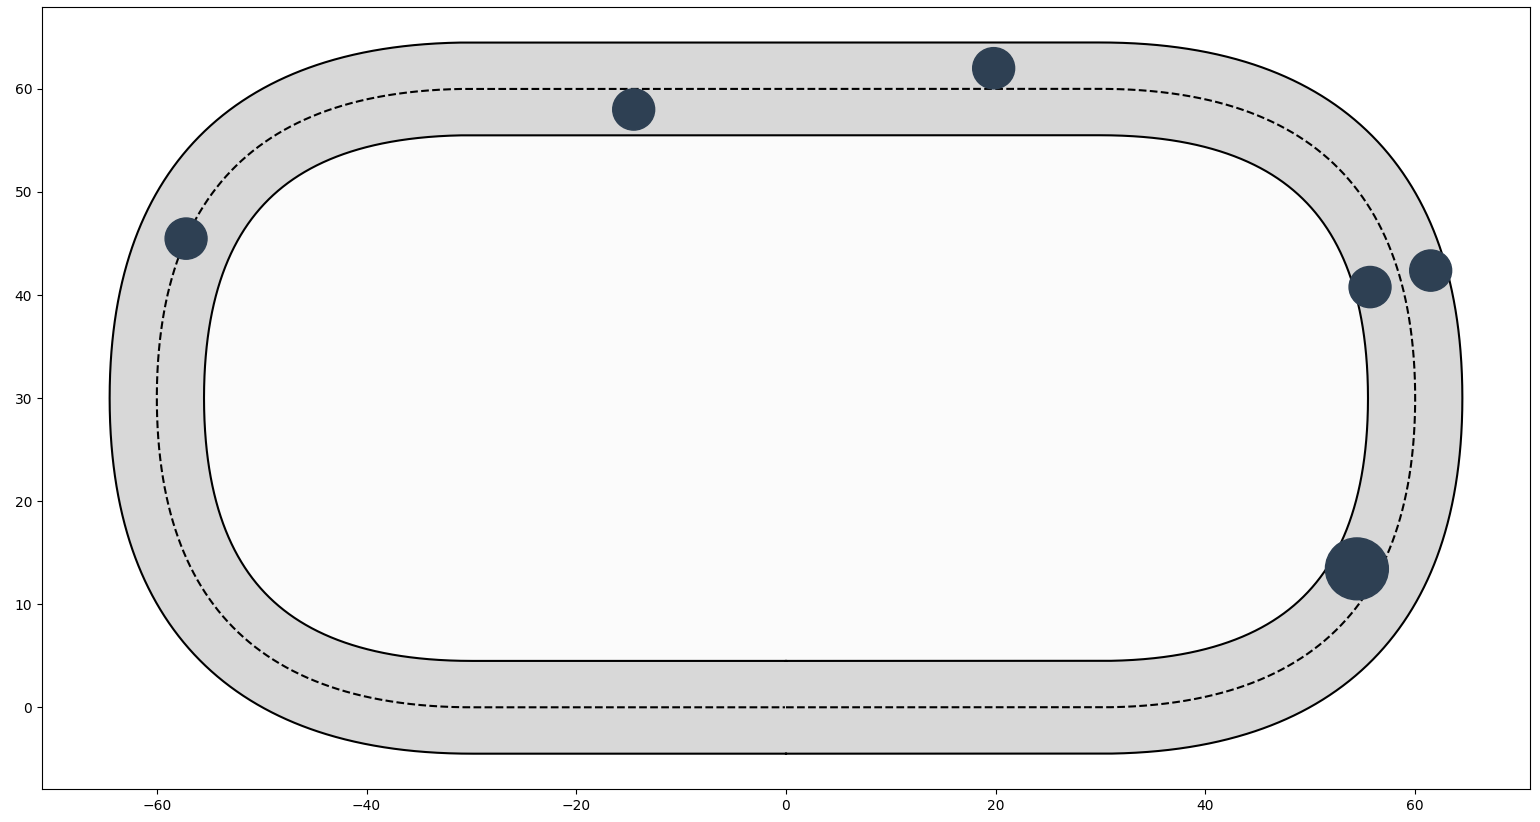
\includegraphics[width=\textwidth]{assets/ippodromo_obstacles.png}
    \caption{Example track}
    \label{ippodromo}
\end{figure}

\subsection{Serially cascaded dynamical model}
While a single control loop system is a simple structure that consists in
just one primary loop that regulates directly the system, the cascade control
makes use of multiple control loops nested within each other. The requirements
for an effective cascade control are that the inner loops variables must be 
faster-responding than the outer ones, and the major disturbances enter in the 
inner loops. Considering the simplest cascade control structure,\\
... (aggiungi schema/equazioni generiche del cascade semplice)

According to the control objectives, a cascade control scheme can include also 
more than one model in its control loops, such that each model capture different
relevant dynamics meeting different control tasks. In this way there is not the 
need to use a high-fidelity model for every objective, because some of them can 
be achieved considering simpler dynamic models. Furthermore, in optimal control
the usage of detailed models for long horizon can bring to an explosion of the 
complexity of the problem; instead, using more detailed models for near terms 
to have a high-fidelity of the real robot, and easier models for planning purpose
in long terms, allows to achieve good performances with computational limits.

When dealing with more than one dynamic model with different dynamic speeds,
the main advantage of a cascade control scheme is the higher performace with respect
to a simple single control loop, thanks to the possibility to control disturbances
in the inner loop before they affect the outer one. The main problem this architecture
can face is in the interaction between the control loops, where the reference signals 
generated by a control loop are not achievable by the others. This happens especially
when we are dealing with models with different complexity levels.

To deal with the disadvantages of the cascade control design, but leveraging on its 
strengths, the idea of \cite{paper} in the scenario of an autonomous car is to build 
a serial architecture which contains two dynamic models, belonging to the same single
control loop and the same prediction horizon. The first one is a single-track vehicle
model, which reflects comprehensively the complex dynamic of the car (we will see in the 
next section the details) and provides all the tools to accurately treat the first
prediction steps. The farthest window of the horizon is treated with a planar point-mass 
model, useful for long-term trajectory planning with low computational resources.
Thus the benefits of the cascade model for the trajectory task are preserved; moreover
the existance of a single control loop ensure the feasibility of the reference targets
that are exchanged between the two models. A very important thing to pay attention is 
in the linkage of the plant models, propagating correctly the final state of the first
model to the initial state of the second model, and mantaining consistency in constraints
and cost functions across interconnected models.


\subsubsection{Single-track dynamic model}
The car can be represented as a dynamic bicycle model, where the two pairs of
front and rear wheels can be merged into a single wheel, one front wheel and one
rear wheel.\\
For the intrinsic properties, the vehicle is assumed to have a mass $\mathbf{m}$
and a yaw moment of inertia $\mathbf{I_{zz}}$; the wheelbase has length
$\mathbf{L}$, divided into $\mathbf{a}$ and $\mathbf{b}$, where they are
respectively the distances between the Center of Gravity and the front and rear
axle; the CG is at a distance $\mathbf{h_{cg}}$ from the ground; the front steer
angle is $\mathbf{\delta}$.\\
Since the model is of second-order, the state is composed of a velocity
component and a position/orientation one. The first one consists of the
longitudinal speed $\mathbf{U_x}$, the lateral speed $\mathbf{U_y}$, and the yaw
rate $\mathbf{r}$ of the CG. Meanwhile, the pose component is expressed in
relative coordinates withe respect to the road descriptor, namely by the
curvilinear coordinate $\mathbf{s}$, the lateral distance $\mathbf{e}$, and the
orientation of the chassis $\mathbf{\Delta \varPsi}$ with respect to the road
descriptor path. The curvature of the path, which is necessary to compute the
curvilinear coordinate and the orientation is called $\mathbf{\kappa}$. Thus, we
can at every time instant identify a unique pose of the vehicle by the tuple
$s,e,\Delta \varPsi$, as already said in section \ref*{subsec:track}.\\
The inputs of the system are the steering angle rate $\dot{\delta}$ and the
total longitudinal force $F_x$. This one can be divided in the longitudinal
force applied on the axle of the front tire $F_{x_f}$ and the longitudinal force
applied on the axle of the rear tire $F_{x_r}$, according to a distribution
function $\tilde{\chi}$:

\begin{equation}
    \tilde{\chi_f} = \frac{d_f - b_f}{2}\tanh(2(F_x+0.5))+\frac{d_f+b_f}{2}
\end{equation}
\begin{equation}
    \tilde{\chi_r} = \frac{b_r-d_r}{2}\tanh(-2(F_x+0.5))+\frac{d_r+b_r}{2}
\end{equation}
where $d_f$ and $d_r$ represent the drive force distribution, and $b_f$ and $b_r$ represent the 
brake force distribution. So the single components of the longitudinal force are:
\begin{equation}
    \tilde{F}_{x_f} = \tilde{\chi}_f(F_x) \cdot F_x
\end{equation}
\begin{equation}
    \tilde{F}_{x_r} = \tilde{\chi}_r(F_x) \cdot F_x
\end{equation}

This implementation might seem rather complex, compared to simply expressing the front and rear force distribution as
\begin{equation}
    \tilde{F}_{x_f} = \tilde{\chi}_f \cdot F_x
\end{equation}
\begin{equation}
    \tilde{F}_{x_r} = \tilde{\chi}_r \cdot F_x
\end{equation}

where $\tilde{\chi}_f$ and $\tilde{\chi}_r$ are scalars that sum to 1, however, these equations will be used for numerical 
optimization, and should therefore be twice differentiable, and we therefore have to use the workaround equations presented above.

For the tire model, given the maximum instantaneous normal load of the tire $F_z$, the maximum possible
lateral tire force that can be obtained applying the input force $\tilde{F}_x$ is:
\begin{equation}
    \tilde{F}_y^{max} = \sqrt[]{(\mu F_z)^2 - (0.99\cdot \tilde{F}_x)^2}
\end{equation}
where $\mu$ is the tire-road friction coefficient and the 99\%  of the longitudinal force is due to solve 
some numerical issues in the optimization problem. \\
The normal loads for the two tires are affected also by the slope $\theta$ of the road, and by the banking $\phi$, in the following way:
\begin{equation}
    \label{normalF}
    F_{z_f} = \frac{b}{L}m(g\cdot \cos(\theta)\cos(\varphi)+A_{V^2}U_x^2)-\frac{h_{cg}}{L}F_x
\end{equation}
\begin{equation}
    \label{normalR}
    F_{z_r} = \frac{a}{L}m(g\cdot \cos(\theta)\cos(\varphi)+A_{V^2}U_x^2)+\frac{h_{cg}}{L}F_x
\end{equation}
where the effect of vertical curvature on speed are expressed through:
\begin{equation}
    A_{V^2} = -\frac{\partial \theta}{\partial s}\cos(\varphi)-\kappa\cdot \sin(\varphi)\cos(\theta) 
\end{equation}
The slip angles of the front ($\alpha_f$) and rear ($\alpha_r$) wheels are respectively given by:
\begin{equation}
    \alpha_f = \arctan \left(\frac{U_y+ar}{U_x}\right)-\delta
\end{equation}
\begin{equation}
    \alpha_r = \arctan \left(\frac{U_y-br}{U_x}\right)
\end{equation}
A full sliding occurs at an angle denoted as $\alpha^{\text{mod}}$, which is calculated as:
\begin{equation}
    \alpha^{\text{mod}} = \arctan\left(\frac{3\cdot F_y^{\text{max}}\cdot\zeta}{C_{\alpha}}\right)
\end{equation}
Here, $\zeta$ is a factor introduced to ensure the tire model's strict monotonicity.\\
Thus, considering $\alpha = \left(\alpha_f \tab \alpha_r\right)^T$, the tire model can
be expressed as:
\begin{equation}
    F_y = 
    \left\{
	\begin{array}{ll}
		-C_\alpha \tan(\alpha)+&\\
        \tabeq\frac{C_\alpha^2}{3\tilde{F}_y^{max}}|\tan(\alpha)|\tan(\alpha) - &\\
        \tabeq\frac{C_\alpha^3}{27(\tilde{F}_{y}^{max})^2}\tan^3(\alpha) 
        & \mbox{if } |\alpha| \leq \alpha^{mod} \\
		-C_{\alpha}(1-2\zeta+\zeta^2)\tan(\alpha)-&\\
        \tabeq \tilde{F}_y^{max}(3\zeta^2-2\zeta^3){sgn(\alpha)}
        & \mbox{otherwise }
	\end{array}
    \right.
\end{equation}
\\
Regarding the drag forces, these are included all in the same variable $F_d$:
\begin{equation}
    \label{drag_force}
    F_d = F_{rr}+C_DU_x^2-mg\sin(\theta)
\end{equation}
where $F_{rr}$ represents the rolling resistance, $C_D$ is the coefficient of aerodynamic
drag. \\
Instead, the lateral force $F_b$ applied on the CG models the effect of the road bank angle $\varphi$:
\begin{equation}
    \label{lateral_force}
    F_b = -mg\cos(\theta)\sin(\varphi)
\end{equation}
\\
\\
All these informations are used to describe the motion of the single-track model:
\begin{equation}
    \dot{U}_x = \frac{F_{x_f}\cos(\delta)-F_{y_f}\sin(\delta)+F_{x_r}-F_d}{m}+rU_y
\end{equation}
\begin{equation}
    \dot{U_y} = \frac{F_{y_f}\cos(\delta)+F_{x_f}\sin(\delta)+F_{y_r}+F_b}{m}-rU_x 
\end{equation}
\begin{equation}
    \dot{r} = \frac{a(F_{y_f}\cos(\delta)+F_{x_f}\sin(\delta))-bF_{y_r}}{I_{zz}}
\end{equation}
\begin{equation}
    \dot{s} = \frac{U_x\cos(\Delta \varPsi) -U_y\sin(\Delta \varPsi)}{1-\kappa e}
\end{equation}
\begin{equation}
    \dot{e} = U_x\sin(\Delta \varPsi)+U_y \cos(\Delta \varPsi)
\end{equation}
\begin{equation}
    \Delta \dot{\varPsi} = r-\kappa \dot{s}
\end{equation}




\subsubsection{Point-Mass model}
The Point-Mass model is a simpler version of the Single-Track model, where the car is approximated with a point object
in the Center of Gravity of the vehicle. Being a one-dimensional object, the point has just one total horizontal velocity state $\bar{V}$, 
and three position states relative to the road descriptor path: the distance $\bar{s}$ along it, the lateral distance $\bar{e}$ from it, and finally the
difference in orientation $\bar{\phi}$ between the velocity vector and the tangent to the road descriptor path.

Substituting ${U}_x$ with $\bar{V}$, we can use some of the equations introduced in the single-track model also for the point-mass model,
in particular for the drag force ${F}_d$ (eq. \ref{drag_force}), for ${F}_b$ (eq. \ref{lateral_force}) and for the normal loads ${F}_{z_f}$ (eq. \ref{normalF}) and ${F}_{z_r}$ (eq. \ref{normalR}).
Following the basic intuition of having to simplify the model, the tire forces are not modeled.

The inputs to this model are the longitudinal force $\bar{F}_x$ and the lateral force $\bar{F}_y$, that are limited by friction limits
according to the following rules:
\begin{equation}
    \left(\frac{b}{L}\bar{F}_y\right)^2 + \left(\tilde{\chi_f}\bar{F}_x\right)^2 \leq \left(\mu_f F_{z_f}\right)^2
\end{equation}
\begin{equation}
    \left(\frac{a}{L}\bar{F}_y\right)^2 + \left(\tilde{\chi_r}\bar{F}_x\right)^2 \leq \left(\mu_r F_{z_r}\right)^2
\end{equation}
Thus the equations that describe the motion of the point-mass model are the following:

\begin{equation}
    \dot{\bar{V}} = \frac{\bar{F}_{x}-\bar{F}_{d}}{m}
\end{equation}
\begin{equation}
    \dot{\bar{s}} = \frac{\bar{V}\cos(\bar{\phi})}{1-\kappa \bar{e}}
\end{equation}
\begin{equation}
    \dot{\bar{e}} = \bar{V}\sin(\bar{\phi})
\end{equation}
\begin{equation}
    \dot{\bar{\phi}} = \frac{{\bar{F}}_y + {\bar{F}}_b}{m\bar{V}} - k\dot{\bar{s}}
\end{equation}

Note that the yaw dynamics are omitted, and therefore this model cannot be used for yaw stabilization

\subsubsection{Propagating the state from single-track to point-mass}
Here we define the mapping from the single-track to the point-mass states. 
It is very important that this mapping is correct, to guarantee that the transition
from one model to the other is compliant to the reality.\\
The mapping is the following:
\begin{equation}
    \bar{V} = \sqrt{U_{x}^{2}-U_{y}^{2}}
\end{equation}
\begin{equation}
    \bar{s} = s
\end{equation}
\begin{equation}
    \bar{e} = e
\end{equation}
\begin{equation}
    \bar{\phi} = arctan\left(\frac{{U}_y}{{U}_x}\right) + \Delta\psi
\end{equation}


\subsection{Spatial dynamics}
The discretization of the models can be done with respect to time or with respect to space, 
according to own purposes. 
Discretizing in time means to divide the time over the horizon in small well-defined time intervals $dt$, 
and leaving the spatial curvilinear coordinate $s$ as an optimization variable in the NLP. This approach
implies to know the temporal window for the horizon.\\ 
Instead, discretizing in space means to establish the spatial discretization steps $ds$ that compose the
total space travelled by the vehicle in the horizon window. In this way the time $t$ can be left as an 
optimization variable.\\
In our scenario, our objective is to minimize the lap time. So the discretization in space is more adapt,
because it allows to minimize the employed time to cover the given space interval. Furthermore, this method
does not allow to the car to stop, fact in which we are not interested in.

\newpage
\section{NLP Structure}

The key element of the NLP is the cost function, for this work we formulate it to minimize time along the finite planning horizon, while also respecting the road boundaries and while keeping the car in a safe configuration. To achieve this, it is composed of the sum of the following seven terms:
\begin{enumerate}
    \item Final time: the time at which the point-mass model reaches the last stage of the planning horizon
    \item Terminal state: to make sure that the final stage is a safe one, we add this penalty based on the lateral position ${\bar{e}}_m$, the course error ${\bar{\phi}}_m$ and the excess speed ${\bar{V}}_{exc}$ of the final stage, with
    \begin{equation}
    {\bar{V}}_{exc} = 
    \left\{
	\begin{array}{ll}
		{\bar{V}}_m - {{\bar{V}}_{safe}}
        & \mbox{if } {\bar{V}}_m > {{\bar{V}}_{safe}} \\
	0 & \mbox{otherwise }
	\end{array}
    \right.
    \end{equation}

    The terms introduced are finally combined in
    
    \begin{equation}{J}_{term} = {W_e}_{term}{\bar{e}}_m^2 + {W_{\phi}}_{term}{\bar{\phi}}_m^2 + {W_V}_{term}{\bar{V}}_{exc}^2
    \end{equation}

    \item Road Boundary Intrusion: we penalize any road excursion
    \begin{equation}
    J_{rb} = W_{rb}\sum_{k=1}^{N} \Delta s_k \begin{cases}
    (e_k - {e_{\text{max}}}_k)^2, & \text{if } e_k \geq e_{\text{max}_k} \\
    (e_k - e_{\text{min}_k})^2, & \text{if } e_k \leq e_{\text{min}_k} \\
    0, & \text{otherwise}
    \end{cases}
    \end{equation}
    \[  + W_{rb}\sum_{l=1}^{M} \Delta\overline{s}_l \begin{cases}
    (\overline{e}_l - \overline{e}_{\text{max}_l})^2, & \text{if } \overline{e}_l \geq \overline{e}_{\text{max}_l} \\
    (\overline{e}_l - \overline{e}_{\text{min}_l})^2, & \text{if } \overline{e}_l \leq \overline{e}_{\text{min}_l} \\
    0, & \text{otherwise}
    \end{cases}
    \]

    where, intuitively, ${e_{\text{max}}}_k$ can be chosen as the width of the road. !!!E' effettivamente cosi? Lo dico ad intuito!!!

    \item Deviation from the Road Descriptor Path: 
    \begin{equation}
    J_{rd} = W_{rd}(\sum_{k=1}^{N} \Delta s_k e_k^2 + \sum_{l=1}^{M} \Delta\overline{s}_l \overline{e}_l^2)
    \end{equation}
    While this might look similar to the previous term, its objective is to increase robustness to any eventual mismatch between models !!!cazzo vordi!!!

    \item Slew rate: in order to encourage smooth controls we penalize too big increases of the steering rate $\dot{\delta}$, variation of the total lateral force $\Delta F_y$, variation of the new commanded longitudinal force ${F_x}_k$ with respect to the previous commanded ${F_x}_{k-1}$.
    And finally, the variation in forces at the model transition, denoted as $\Delta F_u$.
    These are all combined into:
    
    \begin{equation}
        J_{\dot{u}} = J_{\dot{\delta}} + J_{\Delta F_y} + J_{\Delta F_x} + J_{\Delta F_u}
    \end{equation}

    !!!To be completed, vogliamo esprimere le varie J di questo ultimo step o diventa troppo listone di equazioni?!!!
    
    \item Excessive Slip Angle: in order to discourage the car to operate in the fully saturated region of the tires, we add a penalty on excessive slip angle. This helps in stabilizing the car.

    \item Excessive Force Usage Beyond the Imposed Limit:
    To help the optimization problem we introduce some slack variables on the force limits, we introduce this penalty to keep them as small as possible
    
\end{enumerate}

\section{Implementation}

We used as main backbone casadi (\cite{casadi}), a software framework for automatic
differentiation, nonlinear optimization and optimal control. It is implemented
in c++ and has also a python interface. Casadi serves three main purposes:
\begin{itemize}
    \item Modeling
    \item Simulation through numerical integration
    \item Formulation and solving of optimization problems within MPC
\end{itemize}
The modeling part was already addressed, while in this section we will focus
more on the algorithmic perspective. Overall, the simulation loop can be
summarized as follows.

\begin{algorithm}
    \caption{Simulation Loop}\label{sim}
    \begin{algorithmic}[1]
        \State $dt \gets 0.08$ s \Comment{Time step}
        \While{ True }
        \State measure car state $x$
        \State action $a \gets command(x)$ \Comment{From MPC}
        \State move forward for $dt$ under $a$ 
        \EndWhile
    \end{algorithmic}
\end{algorithm}

Line 3 takes the assumption that the state is fully known at each instant. We
take this assumption for simplifying reasons. In a real setting the state would
be measured with sensors and filtering algorithms.

\subsection{MPC Algorithm}
As said, most of the computation happens in the instruction at line 4.

TODO
\begin{itemize}
    \item expansion of command(x) as pseudocode
    \item expansion of "move forward" (integrators)
\end{itemize}


\section{Experiments}


\begin{itemize}
    \item Different configuration scenarios
    \item Results
\end{itemize}



\section{Conclusion}

\begin{itemize}
    \item Take-away message
    \item Pitfalls and future work
\end{itemize}


\newpage
\bibliographystyle{unsrt}
\bibliography{references}

\newpage
\appendix

\section{Details on the track}
\label{app:track}
TODO


\end{document}
